\documentclass[fleqn,10pt,serif,xcolor=dvipsnames]{beamer}

%========================================
% Packages
%========================================

\usepackage{etex}

\usepackage[palatino]{mypackBeamer}

\usepackage{gb4e_micha}

\usepackage{multicol}
\usepackage{pgfplots}

%========================================
% Commands
%========================================

\usepackage{mycommands}

%========================================
% More Layout (Beamer Special)
%========================================

\usetheme[height=0mm]{Rochester}
%\usetheme{Warsaw}


\usecolortheme{dove}

%\useoutertheme[footline=empty,compress,subsection=false]{miniframes}

\usecolortheme[named=Gray]{structure}

\setbeamercolor{title}{fg=Black}

%\setbeamercolor{structure}{fg=Brown}
%\setbeamercolor{normal text}{fg=Brown}
\setbeamercolor{section in head/foot}{bg=gray!20}
%\setbeamercolor{lower separation line head}{bg=black!40}
\setbeamercolor*{frametitle}{fg=Black,bg=gray!20}
\setbeamercolor*{block body}{fg=Black,bg=gray!00}
\setbeamercolor*{block title}{fg=Black,bg=gray!20}
 

% Switch of shadows of boxes
\setbeamertemplate{blocks}[default]

% Frame numbers in footer
\setbeamertemplate{footline}[frame number]

% See-through preview for uncovered
% \setbeamercovered{transparent}

% Switch off navigation panel at bottom right
\beamertemplatenavigationsymbolsempty

% Change Style for itemize markers
% Options are ball, circle, rectangle and default (=triangle)
\setbeamertemplate{items}[circle] 

%\includeonlyframes{current}


\setcounter{tocdepth}{1}

% Use bullets in enumerates and TOC
\setbeamertemplate{enumerate item}[circle]

% Set color for enumerate/TOC bullets to white
\setbeamercolor*{item projected}{fg=Black,bg=gray!00}

%========================================
% Special this document
%========================================

\newcommand{\lit}{\acro{lit}}
\newcommand{\glb}{\acro{glb}}
\newcommand{\loc}{\acro{loc}}

\renewcommand{\AE}{AE}
\newcommand{\GE}{GE}
\newcommand{\LC}{LC}
\newcommand{\EC}{EC}


\newcommand{\mymark}[1]{{\color{blue}{#1}}}

%========================================
% Document
%========================================



\title{Scalar Items in Embedded Position}
\subtitle{An(other) Experimental Approach} 



\author{Petra Augurzky$^1$, Michael Franke$^2$ \& Fabian Schlotterbeck$^3$}
\institute{$^1$ Seminar f\"{u}r Sprachwissenschaft, Universit\"{a}t
  T\"{u}bingen \\
  $^2$ Institute for Logic, Language and Computation, Universiteit van
  Amsterdam\\
  $^3$ Sonderforschungsbereich~833 ``Bedeutungskonstitution'', Universit\"{a}t T\"{u}bingen}
\date{}

% Logo auf allen Folien
% \logo{\pgfimage[height=2cm]{uni-tuebingen-logo.pdf}} 

% Logo auf Titelseite
% \titlegraphic{\pgfimage[height=1.5cm]{unilogo.pdf}}

%--------------------------------------


\begin{document}

% --- Horizontal Space Fix ----

\abovedisplayskip=3pt 
\abovedisplayshortskip=3pt 

\belowdisplayskip=3pt 
\belowdisplayshortskip=3pt 


\begin{frame}[plain]
  \titlepage
\end{frame}

\begin{frame}
  \frametitle{Scalar Items in Embedded Positions \dots}
  \begin{block}{\dots in upward monotonic position}
    \begin{exe}
    \ex \label{bsp:AE} All of the students read some of the
      papers. \hfill (\AE)
    \end{exe}
  \end{block}
  \begin{block}{\dots in non-monotonic position}
    \begin{exe}
    \ex \label{bsp:GE} Exactly one of the students read some of the
      papers. \hfill (\GE)
    \end{exe}
  \end{block}
  \bigskip

  \begin{block}{2 kinds of pragmatic enrichment conceivable:}
    \begin{multicols}{2}
      \begin{itemize}
      \item[(i)] global
      \item[(ii)] local
      \end{itemize}
    \end{multicols}
  \end{block}
\end{frame}

\begin{frame}
  \frametitle{Scalar Items in Embedded Positions}
  \begin{block}{\AE \hfill (Global)}
    \begin{exe}
      \exr{bsp:AE} All of the students read {\color{blue}{some}} of the
      papers.
    \ex All of the students read {\color{blue}{all}} of the papers.
    \ex
      \begin{xlist}
      \ex All of the students read some of the papers and  \\
        not all students read all
        of the papers.
      \ex All read some and at least one did not read all.
      \end{xlist}
    \end{exe}
  \end{block}
  \begin{block}{\AE  \hfill (Local)}
    \begin{exe}
      \exr{bsp:AE} All of the students read {\color{blue}{some}} of the
      papers.
    \ex
      \begin{xlist}
      \ex All of the students read {\color{blue}{some  but not all}} of the papers.
      \ex All read some and no one read all.
      \end{xlist}
    \end{exe}
  \end{block}
\end{frame}


\begin{frame}
  \frametitle{Scalar Items in Embedded Positions}
  \begin{block}{Readings \AE  \hfill (summary)}
    3 kinds of readings:
    \begin{enumerate}
    \item \lit : all \dots some \dots
    \item \glb : all \dots some \dots \& not (all \dots all \dots)
    \item \loc : all \dots some but not all \dots
    \end{enumerate}
    with entailment relations:
    \begin{itemize}
    \item[] \lit\ $\supset$ \glb\ $\supset$ \loc
    \end{itemize}
    distinguishing cases:
    \begin{center}
      \begin{tabular}{lccc}
        \toprule
        & \lit & \glb & \loc \\ \midrule
        false   & 0 & 0 & 0 \\
        literal & 1 & 0 & 0 \\
        weak    & 1 & 1 & 0 \\
        strong  & 1 & 1 & 1 \\ \bottomrule
      \end{tabular}
    \end{center}
  \end{block}
\end{frame}

\begin{frame}
  \frametitle{Scalar Items in Embedded Positions}
  \begin{block}{Distinguishing Cases \AE \hfill (false)}
    
    \medskip 

    \begin{minipage}[c]{0.5\linewidth}
      \vspace{0pt}
      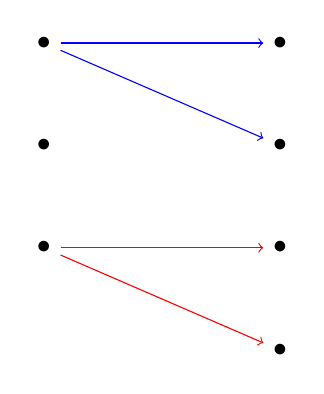
\begin{tikzpicture}[node distance = 1.3cm]
        % Nodes

        \node (X-1) {$\Large{\bullet}$};

        \node (X-2) [below of = X-1] {$\Large{\bullet}$};

        \node (X-3) [below of = X-2] {$\Large{\bullet}$};

        \node (Y-1) [right of = X-1, node distance = 3cm]{$\Large{\bullet}$};

        \node (Y-2) [below of = Y-1] {$\Large{\bullet}$};

        \node (Y-3) [below of = Y-2] {$\Large{\bullet}$};

        \node (Y-4) [below of = Y-3] {$\Large{\bullet}$};

        % Arrows

        \path [draw=blue,->] (X-1) -> (Y-1);

        \path [draw=blue,->] (X-1) -> (Y-2);


        \path [draw=red,->] (X-3) -> (Y-3);

        \path [draw=red,->] (X-3) -> (Y-4);

      \end{tikzpicture}
      \end{minipage}
      \begin{minipage}[c]{0.45\linewidth}
        \vspace{0pt}
    ``All of the dots on the left are connected to some of the dots on
    the right.''
    \medskip

        \begin{itemize}
        \item[] \lit: False
        \item[] \glb: False
        \item[] \loc: False 
        \end{itemize}
      \end{minipage}

  \end{block}
\end{frame}


\begin{frame}
  \frametitle{Scalar Items in Embedded Positions}
  \begin{block}{Distinguishing Cases \AE \hfill (literal)}
    
    \medskip 

    \begin{minipage}[c]{0.5\linewidth}
      \vspace{0pt}
      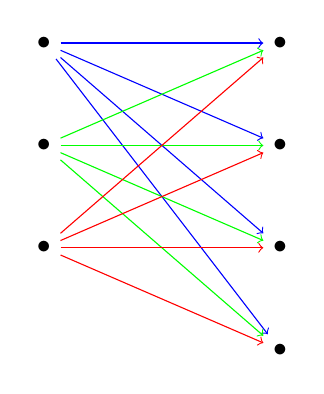
\begin{tikzpicture}[node distance = 1.3cm]
        % Nodes

        \node (X-1) {$\Large{\bullet}$};

        \node (X-2) [below of = X-1] {$\Large{\bullet}$};

        \node (X-3) [below of = X-2] {$\Large{\bullet}$};

        \node (Y-1) [right of = X-1, node distance = 3cm]{$\Large{\bullet}$};

        \node (Y-2) [below of = Y-1] {$\Large{\bullet}$};

        \node (Y-3) [below of = Y-2] {$\Large{\bullet}$};

        \node (Y-4) [below of = Y-3] {$\Large{\bullet}$};

        % Arrows

        \path [draw=blue,->] (X-1) -> (Y-1);

        \path [draw=blue,->] (X-1) -> (Y-2);

        \path [draw=blue,->] (X-1) -> (Y-3);

        \path [draw=blue,->] (X-1) -> (Y-4);


        \path [draw=green,->] (X-2) -> (Y-1);

        \path [draw=green,->] (X-2) -> (Y-2);

        \path [draw=green,->] (X-2) -> (Y-3);

        \path [draw=green,->] (X-2) -> (Y-4);



        \path [draw=red,->] (X-3) -> (Y-1);

        \path [draw=red,->] (X-3) -> (Y-2);

        \path [draw=red,->] (X-3) -> (Y-3);

        \path [draw=red,->] (X-3) -> (Y-4);

      \end{tikzpicture}
      \end{minipage}
      \begin{minipage}[c]{0.45\linewidth}
        \vspace{0pt}
    ``All of the dots on the left are connected to some of the dots on
    the right.''
    \medskip

        \begin{itemize}
        \item[] \lit: True
        \item[] \glb: False
        \item[] \loc: False 
        \end{itemize}
      \end{minipage}

  \end{block}
\end{frame}

\begin{frame}
  \frametitle{Scalar Items in Embedded Positions}
  \begin{block}{Distinguishing Cases \AE \hfill (weak)}
    
    \medskip 

    \begin{minipage}[c]{0.5\linewidth}
      \vspace{0pt}
            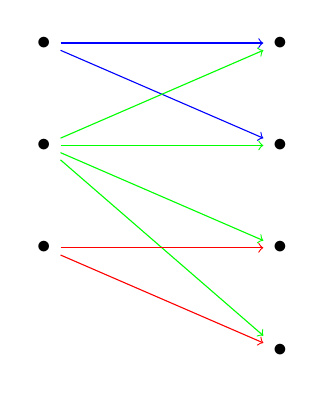
\begin{tikzpicture}[node distance = 1.3cm]
        % Nodes

        \node (X-1) {$\Large{\bullet}$};

        \node (X-2) [below of = X-1] {$\Large{\bullet}$};

        \node (X-3) [below of = X-2] {$\Large{\bullet}$};

        \node (Y-1) [right of = X-1, node distance = 3cm]{$\Large{\bullet}$};

        \node (Y-2) [below of = Y-1] {$\Large{\bullet}$};

        \node (Y-3) [below of = Y-2] {$\Large{\bullet}$};

        \node (Y-4) [below of = Y-3] {$\Large{\bullet}$};

        % Arrows

        \path [draw=blue,->] (X-1) -> (Y-1);

        \path [draw=blue,->] (X-1) -> (Y-2);


        \path [draw=green,->] (X-2) -> (Y-1);

        \path [draw=green,->] (X-2) -> (Y-2);

        \path [draw=green,->] (X-2) -> (Y-3);

        \path [draw=green,->] (X-2) -> (Y-4);


        \path [draw=red,->] (X-3) -> (Y-3);

        \path [draw=red,->] (X-3) -> (Y-4);

      \end{tikzpicture}
      \end{minipage}
      \begin{minipage}[c]{0.45\linewidth}
        \vspace{0pt}
    ``All of the dots on the left are connected to some of the dots on
    the right.''
    \medskip

        \begin{itemize}
        \item[] \lit: True
        \item[] \glb: True
        \item[] \loc: False 
        \end{itemize}
      \end{minipage}

  \end{block}
\end{frame}


\begin{frame}
  \frametitle{Scalar Items in Embedded Positions}
  \begin{block}{Distinguishing Cases \AE \hfill (strong)}
    
    \medskip 

    \begin{minipage}[c]{0.5\linewidth}
      \vspace{0pt}
            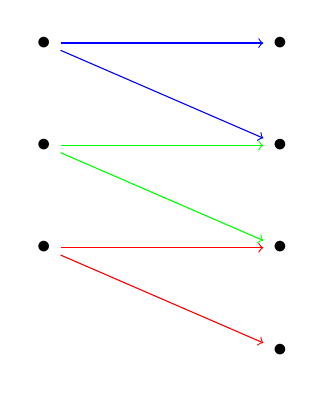
\begin{tikzpicture}[node distance = 1.3cm]
        % Nodes

        \node (X-1) {$\Large{\bullet}$};

        \node (X-2) [below of = X-1] {$\Large{\bullet}$};

        \node (X-3) [below of = X-2] {$\Large{\bullet}$};

        \node (Y-1) [right of = X-1, node distance = 3cm]{$\Large{\bullet}$};

        \node (Y-2) [below of = Y-1] {$\Large{\bullet}$};

        \node (Y-3) [below of = Y-2] {$\Large{\bullet}$};

        \node (Y-4) [below of = Y-3] {$\Large{\bullet}$};

        % Arrows

        \path [draw=blue,->] (X-1) -> (Y-1);

        \path [draw=blue,->] (X-1) -> (Y-2);


        \path [draw=green,->] (X-2) -> (Y-2);

        \path [draw=green,->] (X-2) -> (Y-3);


        \path [draw=red,->] (X-3) -> (Y-3);

        \path [draw=red,->] (X-3) -> (Y-4);

      \end{tikzpicture}
      \end{minipage}
      \begin{minipage}[c]{0.45\linewidth}
        \vspace{0pt}
    ``All of the dots on the left are connected to some of the dots on
    the right.''
    \medskip

        \begin{itemize}
        \item[] \lit: True
        \item[] \glb: True
        \item[] \loc: True 
        \end{itemize}
      \end{minipage}

  \end{block}
\end{frame}

%%%%%%%%%%%%%%%%%%%%%%%%%%%%%%%%%%%%%%%%%%%%%%%%%%
%%%%% Non-Monotonic
%%%%%%%%%%%%%%%%%%%%%%%%%%%%%%%%%%%%%%%%%%%%%%%%%%

\begin{frame}[shrink=2]
  \frametitle{Scalar Items in Embedded Positions}
  \begin{block}{\GE \hfill (Global)}
    \begin{exe}
      \exr{bsp:GE} Exactly one of the students read {\color{blue}{some}} of the
      papers.
    \ex Exactly one of the students read {\color{blue}{all}} of the papers.
    \ex
      \begin{xlist}
      \ex Exactly one of the students read some and  \\
        it's not the case that exactly one read all.
      \ex Exactly one student read some but not all and  \\
        no one else read anything.
      \end{xlist}
    \end{exe}
  \end{block}
  \begin{block}{\GE \hfill (Local)}
    \begin{exe}
      \exr{bsp:GE} Exactly one of the students read {\color{blue}{some}} of the
      papers.
    \ex
      \begin{xlist}
      \ex Exactly one of the students read {\color{blue}{some but not all}} of the papers.
      \ex Exactly one student read some but not all and  \\
        all of the others read all or nothing.
      \end{xlist}
    \end{exe}
  \end{block}
\end{frame}


\begin{frame}
  \frametitle{Scalar Items in Embedded Positions}
  \begin{block}{Reading GE \hfill (summary)}
    3 kinds of readings:
    \begin{enumerate}
    \item \lit: exactly one \dots some \dots
    \item \glb: exactly one \dots some \dots \& not (exactly one \dots all \dots)
    \item \loc: exactly one \dots some but not all \dots
    \end{enumerate}
    with entailment relations:
    \vspace{-0.3cm}
    \begin{multicols}{2}
      \begin{itemize}
      \item[] \lit\ $\supset$ \glb\ $\color{blue}{\subset}$ \loc
      \item[] \lit\ $\not \supset$ \loc
      \end{itemize}
    \end{multicols}
    \vspace{-0.15cm}
    distinguishing cases:
    \begin{center}
      \begin{tabular}{lccc}
      \toprule
      & \textsc{lit} & \textsc{glb} & \textsc{loc} \\ \midrule
      false   & 0 & 0 & 0 \\
      literal & 1 & 0 & 0 \\
      local   & 0 & 0 & 1 \\
      all     & 1 & 1 & 1 \\ \bottomrule
    \end{tabular}
    \end{center}
  \end{block}
\end{frame}


\begin{frame}
  \frametitle{Scalar Items in Embedded Positions}
  \begin{block}{Distinguishing Cases \GE \hfill (false)}
    
    \medskip 
    \begin{minipage}[c]{0.5\linewidth}
      \vspace{0pt}
    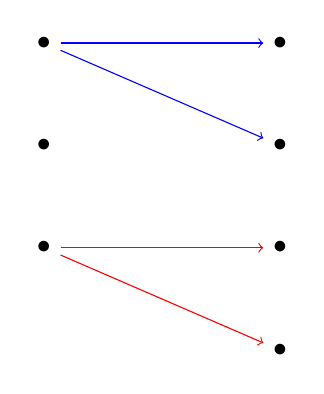
\begin{tikzpicture}[node distance = 1.3cm]
        % Nodes

        \node (X-1) {$\Large{\bullet}$};

        \node (X-2) [below of = X-1] {$\Large{\bullet}$};

        \node (X-3) [below of = X-2] {$\Large{\bullet}$};

        \node (Y-1) [right of = X-1, node distance = 3cm]{$\Large{\bullet}$};

        \node (Y-2) [below of = Y-1] {$\Large{\bullet}$};

        \node (Y-3) [below of = Y-2] {$\Large{\bullet}$};

        \node (Y-4) [below of = Y-3] {$\Large{\bullet}$};

        % Arrows

        \path [draw=blue,->] (X-1) -> (Y-1);

        \path [draw=blue,->] (X-1) -> (Y-2);


        \path [draw=red,->] (X-3) -> (Y-3);

        \path [draw=red,->] (X-3) -> (Y-4);

      \end{tikzpicture}
    \end{minipage}
    \begin{minipage}[c]{0.45\linewidth}
        \vspace{0pt}
    ``Exactly one of the dots on the left are connected to some of the dots on
    the right.''
    \medskip

        \begin{itemize}
        \item[] \lit: False
        \item[] \glb: False
        \item[] \loc: False 
        \end{itemize}
      \end{minipage}

  \end{block}
\end{frame}

\begin{frame}
  \frametitle{Scalar Items in Embedded Positions}
  \begin{block}{Distinguishing Cases \GE \hfill (lit)}
    
    \medskip 

    \begin{minipage}[c]{0.5\linewidth}
      \vspace{0pt}
      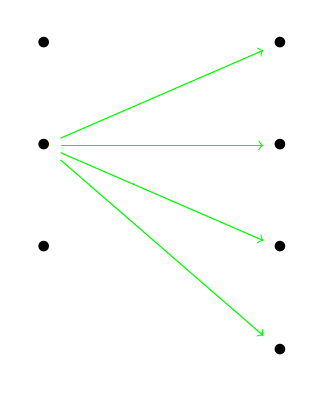
\begin{tikzpicture}[node distance = 1.3cm]
        % Nodes

        \node (X-1) {$\Large{\bullet}$};

        \node (X-2) [below of = X-1] {$\Large{\bullet}$};

        \node (X-3) [below of = X-2] {$\Large{\bullet}$};

        \node (Y-1) [right of = X-1, node distance = 3cm]{$\Large{\bullet}$};

        \node (Y-2) [below of = Y-1] {$\Large{\bullet}$};

        \node (Y-3) [below of = Y-2] {$\Large{\bullet}$};

        \node (Y-4) [below of = Y-3] {$\Large{\bullet}$};

        % Arrows

        \path [draw=green,->] (X-2) -> (Y-1);

        \path [draw=green,->] (X-2) -> (Y-2);

        \path [draw=green,->] (X-2) -> (Y-3);

        \path [draw=green,->] (X-2) -> (Y-4);

      \end{tikzpicture}
      \end{minipage}
      \begin{minipage}[c]{0.45\linewidth}
        \vspace{0pt}
    ``Exactly one of the dots on the left are connected to some of the dots on
    the right.''
    \medskip

        \begin{itemize}
        \item[] \lit: True
        \item[] \glb: False
        \item[] \loc: False 
        \end{itemize}
      \end{minipage}

  \end{block}
\end{frame}


\begin{frame}
  \frametitle{Scalar Items in Embedded Positions}
  \begin{block}{Distinguishing Cases \GE \hfill (loc)}
    
    \medskip 

    \begin{minipage}[c]{0.5\linewidth}
      \vspace{0pt}
            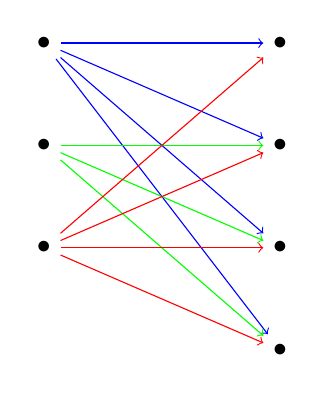
\begin{tikzpicture}[node distance = 1.3cm]
        % Nodes

        \node (X-1) {$\Large{\bullet}$};

        \node (X-2) [below of = X-1] {$\Large{\bullet}$};

        \node (X-3) [below of = X-2] {$\Large{\bullet}$};

        \node (Y-1) [right of = X-1, node distance = 3cm]{$\Large{\bullet}$};

        \node (Y-2) [below of = Y-1] {$\Large{\bullet}$};

        \node (Y-3) [below of = Y-2] {$\Large{\bullet}$};

        \node (Y-4) [below of = Y-3] {$\Large{\bullet}$};

        % Arrows

        \path [draw=blue,->] (X-1) -> (Y-1);

        \path [draw=blue,->] (X-1) -> (Y-2);

        \path [draw=blue,->] (X-1) -> (Y-3);

        \path [draw=blue,->] (X-1) -> (Y-4);



        \path [draw=green,->] (X-2) -> (Y-2);

        \path [draw=green,->] (X-2) -> (Y-3);

        \path [draw=green,->] (X-2) -> (Y-4);



        \path [draw=red,->] (X-3) -> (Y-1);

        \path [draw=red,->] (X-3) -> (Y-2);

        \path [draw=red,->] (X-3) -> (Y-3);

        \path [draw=red,->] (X-3) -> (Y-4);

      \end{tikzpicture}
      \end{minipage}
      \begin{minipage}[c]{0.45\linewidth}
        \vspace{0pt}
    ``All of the dots on the left are connected to some of the dots on
    the right.''
    \medskip

        \begin{itemize}
        \item[] \lit: False
        \item[] \glb: False
        \item[] \loc: True 
        \end{itemize}
      \end{minipage}

  \end{block}
\end{frame}


\begin{frame}
  \frametitle{Scalar Items in Embedded Positions}
  \begin{block}{Distinguishing Cases \GE \hfill (all)}
    
    \medskip 

    \begin{minipage}[c]{0.5\linewidth}
      \vspace{0pt}
      \begin{tikzpicture}[node distance = 1.3cm]
        % Nodes

        \node (X-1) {$\Large{\bullet}$};

        \node (X-2) [below of = X-1] {$\Large{\bullet}$};

        \node (X-3) [below of = X-2] {$\Large{\bullet}$};

        \node (Y-1) [right of = X-1, node distance = 3cm]{$\Large{\bullet}$};

        \node (Y-2) [below of = Y-1] {$\Large{\bullet}$};

        \node (Y-3) [below of = Y-2] {$\Large{\bullet}$};

        \node (Y-4) [below of = Y-3] {$\Large{\bullet}$};

        % Arrows

        \path [draw=blue,->] (X-1) -> (Y-1);

        \path [draw=blue,->] (X-1) -> (Y-2);

      \end{tikzpicture}
      \end{minipage}
      \begin{minipage}[c]{0.45\linewidth}
        \vspace{0pt}
    ``All of the dots on the left are connected to some of the dots on
    the right.''
    \medskip

        \begin{itemize}
        \item[] \lit: True
        \item[] \glb: True
        \item[] \loc: True 
        \end{itemize}
      \end{minipage}

  \end{block}
\end{frame}

\begin{frame}
  \frametitle{Relevance}
  \begin{block}{Is there a local reading?}
    \begin{itemize}
    \item if ``some'' can be enriched locally, it is questionable
      whether this can be explained as a normal scalar implicature in
      the vein of Grice
      \begin{itemize}
        \item local reading in \GE-condition makes sentence literally false
      \end{itemize}
    \item in that case we need to find a different satisfactory and
      systematic explanation
      \begin{itemize}
       \item e.g.~\citet{Chierchia:2004_ScalarImplicatures},  \citet{ChierchiaFox2008:The-Grammatical}
      \end{itemize}

    \end{itemize}
  \end{block}
\end{frame}

\begin{frame}
  \frametitle{Overview}
  brief summary:
  \begin{enumerate}
  \item \citet{GeurtsPouscoulous2009:Embedded-Implic}
  \item \citet{ChemlaSpector2010:Experimental-Ev}
  \item ``K1''
  \end{enumerate}
\end{frame}

\begin{frame}
  \frametitle{Experimental Study 1:
    \citet{GeurtsPouscoulous2009:Embedded-Implic}}
  \begin{minipage}[t]{0.6\linewidth}
    \vspace{0cm}
      \begin{itemize}
      \item picture verification task
      \item critical sentences (in Dutch):
        \begin{enumerate}
        \item[\AE] All the squares are connected with some of the
          circles. 
        \item[\GE] Exactly two squares are connected with some of the
          circles. 
        \end{enumerate}
      \item critical pictures:
        \begin{itemize}
        \item[] \AE-weak: \lit\ = \glb = 1; \loc\ = 0
        \item[] \GE-local: \lit\ = \glb = 0; \loc = 1
        \end{itemize}
      \item results: no \loc-responses \emph{at all}!
        \begin{itemize}
        \item in \AE-weak unanimously ``true''
        \item in \GE-local unanimously ``false''
        \end{itemize}
      \end{itemize}
  \end{minipage}
  \hspace{0.1cm}
  \begin{minipage}[t]{0.35\linewidth}
    \vspace{0cm}
    \begin{flushright}
      \includegraphics[scale=0.35]{Geurts_Pouscoulous_2009_ExpItem.png}
    \end{flushright}
      \vspace{-0.5cm}
      \begin{center}
        \acro{ae}-weak
      \end{center}
  \end{minipage}
\end{frame}

\begin{frame}
  \frametitle{Experimental Study 2:
    \citet{ChemlaSpector2010:Experimental-Ev}}
  \begin{minipage}[t]{0.6\linewidth}
    \vspace{0cm}
      \begin{itemize}
      \item ``picture rating task'':
        \begin{itemize}
        \item continuous \acro{tv}-judgements
        \end{itemize}
      \item critical sentences:
        \begin{enumerate}
        \item[\AE] Chaque lettre est reli\'{e}e \`{a} certains de ses cercles.
        \item[\GE] Il y a exactement une lettre reli\'{e}e \`{a}
          certains de ses cercles.
        \end{enumerate}
      \item critical pictures:
        \begin{itemize}
        \item[] \AE-weak: \lit\ = \glb = 1; \loc\ = 0
        \item[] \GE-local: \lit\ = \glb = 0; \loc = 1
        \end{itemize}
      \item results: attested \loc-responses!
      \end{itemize}
  \end{minipage}
  \hspace{0.1cm}
  \begin{minipage}[t]{0.35\linewidth}
    \vspace{0cm}
    \begin{center}
      \includegraphics[scale=0.25]{Chemla_Spector_2010_Critical_AE.png}\\
      \includegraphics[scale=0.25]{Chemla_Spector_2010_RatingBar.png}
    \end{center}
      \vspace{-0.5cm}
      \begin{center}
        \acro{ae}-weak
      \end{center}
  \end{minipage}
\end{frame}

\begin{frame}
  \frametitle{Experimental Study 2:
    \citet{ChemlaSpector2010:Experimental-Ev}}
  \begin{block}{Results \acro{ae}}
    \medskip
    \includegraphics[width=6.5cm]{Chemla_Spector_2010_ExpItem.png}
    \includegraphics[width=4.5cm]{Chemla_Spector_2010_Results_AE.png}
    \medskip
    \begin{center}
      ``Each letter is connected to some of its circles.''
    \end{center}
  \end{block}
\end{frame}


\begin{frame}
  \frametitle{Experimental Study 2:
    \citet{ChemlaSpector2010:Experimental-Ev}}
  \begin{block}{Results \acro{ge}}
    \medskip
    \includegraphics[width=6.5cm]{Chemla_Spector_2010_ExpItem_GE.png}
    \includegraphics[width=4.5cm]{Chemla_Spector_2010_Results_GE.png}
    \medskip
    \begin{center}
      ``Exactly one letter is connected to some of its circles.''
    \end{center}
  \end{block}
\end{frame}

\begin{frame}
  \frametitle{Experimental Study 3: ``K1''}
  \begin{minipage}[t]{0.6\linewidth}
    \vspace{0cm}
      \begin{itemize}
      \item picture verification task
      \item critical sentences:
        \begin{enumerate}
        \item[\AE] F\"{u}r jeden dieser Umweltsch\"{u}tzer gilt: er
          boykottierte einige dieser Gro\ss konzerne.
        \item[\GE] F\"{u}r genau einen dieser Umweltsch\"{u}tzer gilt:
          er boykottierte einige dieser Gro\ss konzerne.
        \end{enumerate}
      \item critical pictures:
        \begin{itemize}
        \item[] \AE-weak: \lit\ = \glb = 1; \loc\ = 0
        \item[] \GE-local: \lit\ = \glb = 0; \loc = 1
        \end{itemize}
      \item results: significant \loc-responses
      \end{itemize}
  \end{minipage}
  \hspace{0.1cm}
  \begin{minipage}[t]{0.35\linewidth}
    \vspace{0cm}
    \begin{flushright}
      \includegraphics[width=3.8cm]{./../../pictures/Umweltschuetzer02.PNG}
      \vspace{-0.7cm}
      \begin{center}
        \acro{ae}-weak
      \end{center}
      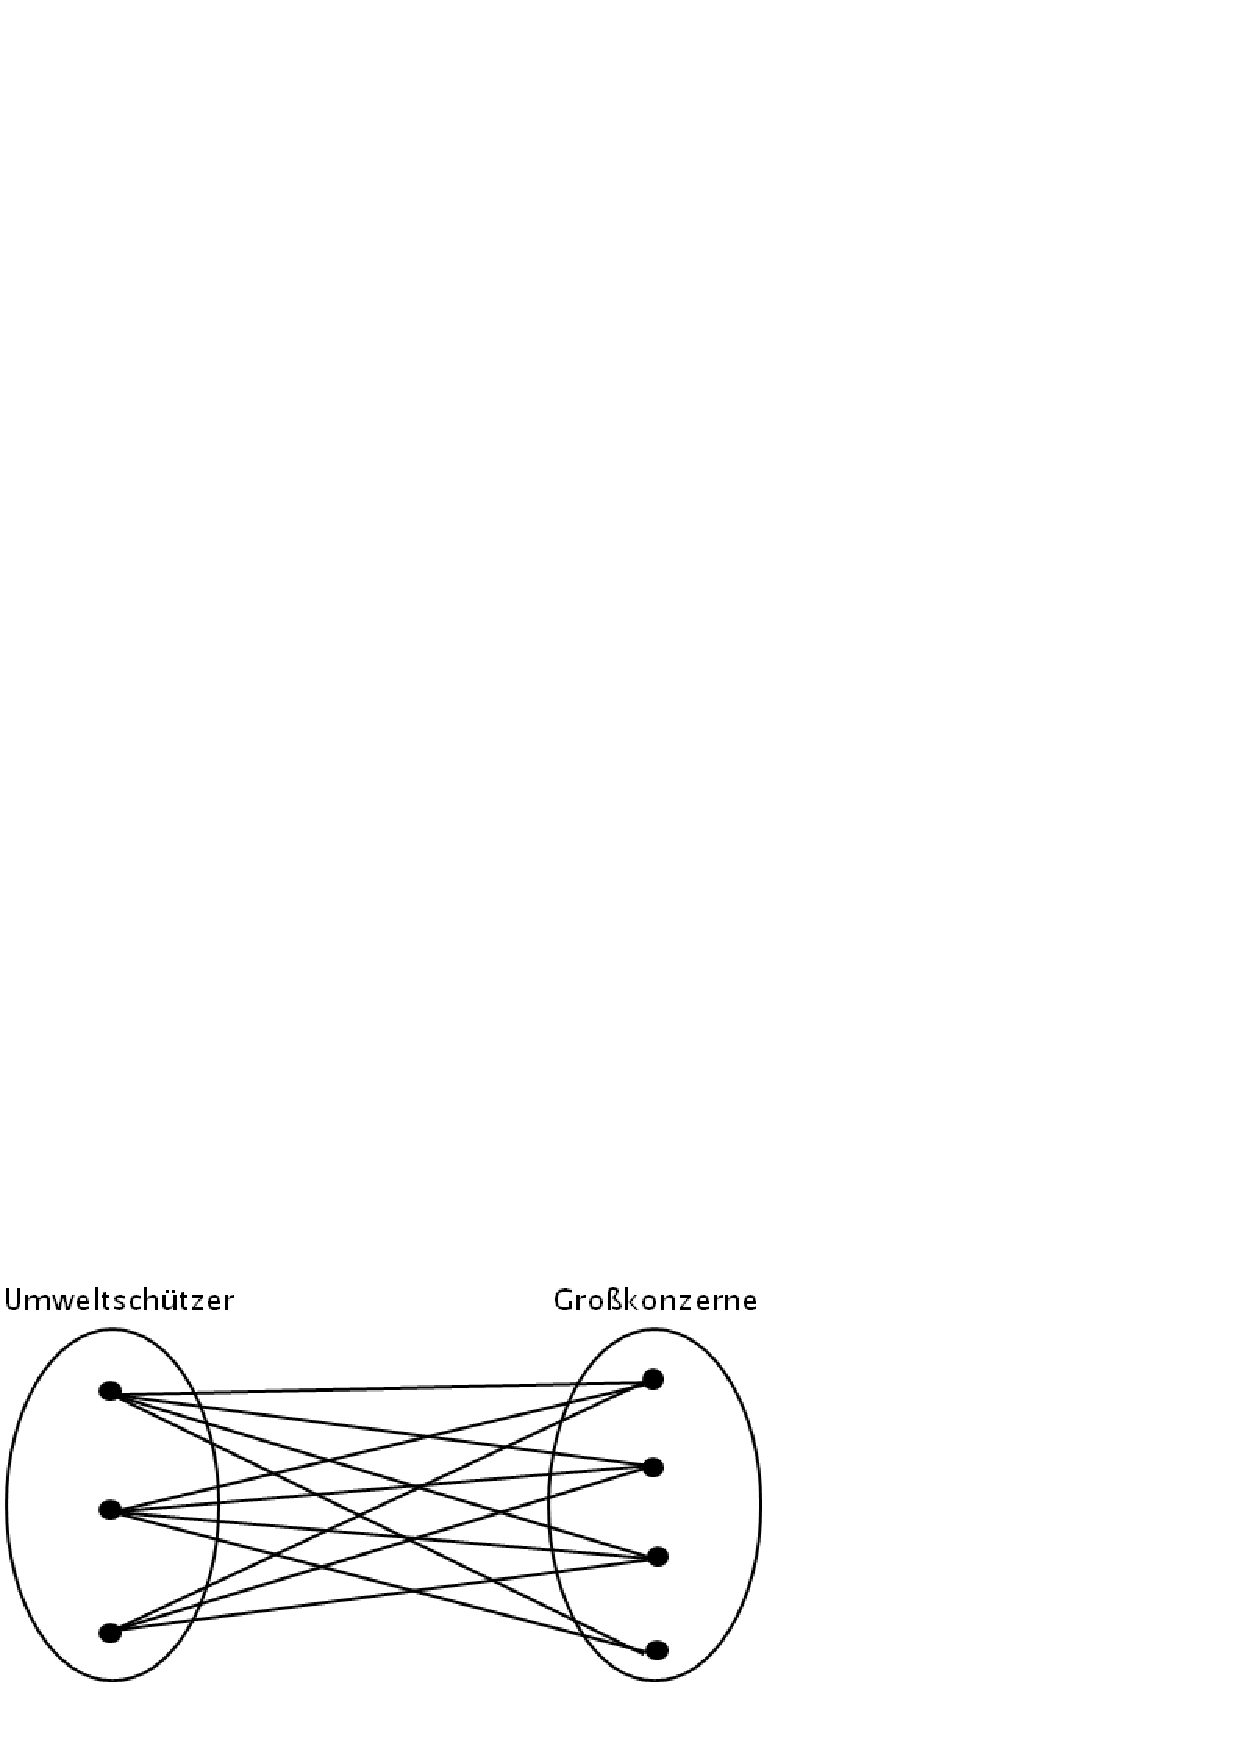
\includegraphics[width=4cm]{./../../pictures/Umweltschuetzer06.PNG}
      \vspace{-0.7cm}
      \begin{center}
        \acro{ge}-local
      \end{center}
    \end{flushright}
  \end{minipage}
\end{frame}


\begin{frame}
  \frametitle{Experimental Study 3: ``K1''}
  \begin{block}{Results}
    \begin{minipage}[t]{0.45\linewidth}
      \vspace{0cm}
      \includegraphics[scale=0.3]{K1_Results_AE.png}
      \vspace{-0.6cm}
      \begin{center}
        \acro{ae}-condition
      \end{center}
    \end{minipage}
    \hspace{0.3cm}
    \begin{minipage}[t]{0.45\linewidth}
      \vspace{0cm}
      \includegraphics[scale=0.3]{K1_Results_GE.png}
      \vspace{-0.6cm}
      \begin{center}
        \acro{ge}-condition
      \end{center}
    \end{minipage}
  \end{block}
\end{frame}

\begin{frame}
  \frametitle{Reflection}
  
  \begin{block}{Conclusion}
    contradictory evidence for/against existence of \loc-readings
  \end{block}
  
  \begin{block}{Potential Problem}
    truth-value judgement/rating tasks make it impossible to separate:
      \begin{enumerate}
      \item availability of a reading
      \item picture~complexity/stereotypicality
      \end{enumerate}

  \end{block}

\end{frame}


\begin{frame}
  \frametitle{Overview: K2}
  \begin{block}{Design}
    \begin{itemize}
    \item visually-incremental \acro{tv}-judgement task
    \item auditory presentation to study effect on prosodic stress on
      scalar item
    \end{itemize}
  \end{block}
  \begin{block}{Results}
    \begin{itemize}
    \item local readings attested but dispreferred
    \item no effect of prosodic stress
    \end{itemize}
  \end{block}
\end{frame}

\begin{frame}
  \frametitle{Overview: K2}
  \begin{block}{Conditions}
    \begin{enumerate}
    \item target
    \item target-related fillers
    \item fillers
    \item controls
    \end{enumerate}
  \end{block}

  \begin{block}{Target Conditions}
      \begin{center}
        \begin{tabular}{cll}
          & \multicolumn{2}{c}{prosody-type} \\ 
          sentence-type & neutral & accented \\ \midrule
          \AE & ae-ntr & ae-acc \\
          \GE & ge-ntr & ge-acc\\
        \end{tabular}
      \end{center}
  \end{block}

\end{frame}


\begin{frame}
  \frametitle{\AE-Sequence}
  \begin{center}
    ``Alle diese Briefe sind mit einigen ihrer Dreiecke verbunden.''

    \vspace{0.1cm}

    \includegraphics[width=0.5 \textwidth]{../../pictures/ae_01_1.pdf}

    \vspace{0.1cm}

    \begin{multicols}{3}
      \begin{itemize} 
      \item[$\Box$] True\\
        \onslide<2>{$\leadsto$  \mymark{false}}
      \item[$\Box$] False\\
        \onslide<2>{$\leadsto$ \mymark{false}}
      \item[$\Box$] Need more info 
      \end{itemize}
    \end{multicols}

  \end{center}
\end{frame}

\begin{frame}
  \frametitle{\AE-Sequence}
  \begin{center}
    ``Alle diese Briefe sind mit einigen ihrer Dreiecke verbunden.''

    \vspace{0.1cm}

    \includegraphics[width=0.5 \textwidth]{../../pictures/ae_01_2.pdf}

    \vspace{0.1cm}

    \begin{multicols}{3}
      \begin{itemize} 
      \item[$\Box$] True\\
        \onslide<2>{$\leadsto$  \mymark{false}}
      \item[$\Box$] False\\
        \onslide<2>{$\leadsto$ \mymark{false}}
      \item[$\Box$] Need more info 
      \end{itemize}
    \end{multicols}

  \end{center}
\end{frame}

\begin{frame}
  \frametitle{\AE-Sequence}
  \begin{center}
    ``Alle diese Briefe sind mit einigen ihrer Dreiecke verbunden.''

    \vspace{0.1cm}

    \includegraphics[width=0.5 \textwidth]{../../pictures/ae_01_3.pdf}

    \vspace{0.1cm}

    \begin{multicols}{3}
      \begin{itemize} 
      \item[$\Box$] True\\
        \onslide<2>{$\leadsto$  \mymark{literal}}
      \item[$\Box$] False\\
        \onslide<2>{$\leadsto$ \mymark{false}}
      \item[$\Box$] Need more info 
      \end{itemize}
    \end{multicols}

  \end{center}
\end{frame}

\begin{frame}
  \frametitle{\AE-Sequence}
  \begin{center}
    ``Alle diese Briefe sind mit einigen ihrer Dreiecke verbunden.''

    \vspace{0.1cm}

    \includegraphics[width=0.5 \textwidth]{../../pictures/ae_01_4.pdf}

    \vspace{0.1cm}

    \begin{multicols}{3}
      \begin{itemize} 
      \item[$\Box$] True\\
        \onslide<2>{$\leadsto$  \mymark{false}}
      \item[$\Box$] False\\
        \onslide<2>{$\leadsto$ \mymark{false}}
      \item[$\Box$] Need more info 
      \end{itemize}
    \end{multicols}

  \end{center}
\end{frame}
\begin{frame}
  \frametitle{\AE-Sequence}
  \begin{center}
    ``Alle diese Briefe sind mit einigen ihrer Dreiecke verbunden.''

    \vspace{0.1cm}

    \includegraphics[width=0.5 \textwidth]{../../pictures/ae_01_5.pdf}

    \vspace{0.1cm}

    \begin{multicols}{3}
      \begin{itemize} 
      \item[$\Box$] True\\
        \onslide<2>{$\leadsto$  \mymark{global}}
      \item[$\Box$] False\\
        \onslide<2>{$\leadsto$ \mymark{false}}
      \item[$\Box$] Need more info 
      \end{itemize}
    \end{multicols}

  \end{center}
\end{frame}


\begin{frame}
  \frametitle{\AE-Sequence}
  \begin{center}
    ``Alle diese Briefe sind mit einigen ihrer Dreiecke verbunden.''

    \vspace{0.1cm}

    \includegraphics[width=0.5 \textwidth]{../../pictures/ae_01_6.pdf}

    \vspace{0.1cm}

    \begin{multicols}{3}
      \begin{itemize} 
      \item[$\Box$] True\\
        \onslide<2>{$\leadsto$  \mymark{false}}
      \item[$\Box$] False\\
        \onslide<2>{$\leadsto$ \mymark{false}}
      \item[$\Box$] Need more info 
      \end{itemize}
    \end{multicols}

  \end{center}
\end{frame}

\begin{frame}
  \frametitle{\AE-Sequence}
  \begin{center}
    ``Alle diese Briefe sind mit einigen ihrer Dreiecke verbunden.''

    \vspace{0.1cm}

    \includegraphics[width=0.5 \textwidth]{../../pictures/ae_01_7.pdf}

    \vspace{0.1cm}

    \begin{multicols}{3}
      \begin{itemize} 
      \item[$\Box$] True\\
        \onslide<2>{$\leadsto$  \mymark{false}}
      \item[$\Box$] False\\
        \onslide<2>{$\leadsto$ \mymark{local}}
      \item[$\Box$] Need more info 
      \end{itemize}
    \end{multicols}

  \end{center}
\end{frame}

\begin{frame}
  \frametitle{\GE-Sequence}
  \begin{center}
    ``Genau eine der Glocken ist mit einigen ihrer Halbkreise verbunden.''

    \vspace{0.1cm}

    \includegraphics[width=0.5 \textwidth]{../../pictures/ge_01_1.pdf}

    \vspace{0.1cm}

    \begin{multicols}{3}
      \begin{itemize} 
      \item[$\Box$] True\\
        \onslide<2>{$\leadsto$  \mymark{false}}
      \item[$\Box$] False\\
        \onslide<2>{$\leadsto$ \mymark{false}}
      \item[$\Box$] Need more info 
      \end{itemize}
    \end{multicols}

  \end{center}
\end{frame}


\begin{frame}
  \frametitle{\GE-Sequence}
  \begin{center}
    ``Genau eine der Glocken ist mit einigen ihrer Halbkreise verbunden.''

    \vspace{0.1cm}

    \includegraphics[width=0.5 \textwidth]{../../pictures/ge_01_2.pdf}

    \vspace{0.1cm}

    \begin{multicols}{3}
      \begin{itemize} 
      \item[$\Box$] True\\
        \onslide<2>{$\leadsto$  \mymark{false}}
      \item[$\Box$] False\\
        \onslide<2>{$\leadsto$ \mymark{global}}
      \item[$\Box$] Need more info 
      \end{itemize}
    \end{multicols}

  \end{center}
\end{frame}

\begin{frame}
  \frametitle{\GE-Sequence}
  \begin{center}
    ``Genau eine der Glocken ist mit einigen ihrer Halbkreise verbunden.''

    \vspace{0.1cm}

    \includegraphics[width=0.5 \textwidth]{../../pictures/ge_01_3.pdf}

    \vspace{0.1cm}

    \begin{multicols}{3}
      \begin{itemize} 
      \item[$\Box$] True\\
        \onslide<2>{$\leadsto$  \mymark{false}}
      \item[$\Box$] False\\
        \onslide<2>{$\leadsto$ \mymark{literal}}
      \item[$\Box$] Need more info 
      \end{itemize}
    \end{multicols}

  \end{center}
\end{frame}

\begin{frame}
  \frametitle{\GE-Sequence}
  \begin{center}
    ``Genau eine der Glocken ist mit einigen ihrer Halbkreise verbunden.''

    \vspace{0.1cm}

    \includegraphics[width=0.5 \textwidth]{../../pictures/ge_01_4.pdf}

    \vspace{0.1cm}

    \begin{multicols}{3}
      \begin{itemize} 
      \item[$\Box$] True\\
        \onslide<2>{$\leadsto$  \mymark{false}}
      \item[$\Box$] False\\
        \onslide<2>{$\leadsto$ \mymark{false}}
      \item[$\Box$] Need more info 
      \end{itemize}
    \end{multicols}

  \end{center}
\end{frame}

\begin{frame}
  \frametitle{\GE-Sequence}
  \begin{center}
    ``Genau eine der Glocken ist mit einigen ihrer Halbkreise verbunden.''

    \vspace{0.1cm}

    \includegraphics[width=0.5 \textwidth]{../../pictures/ge_01_5.pdf}

    \vspace{0.1cm}

    \begin{multicols}{3}
      \begin{itemize} 
      \item[$\Box$] True\\
        \onslide<2>{$\leadsto$  \mymark{local}}
      \item[$\Box$] False\\
        \onslide<2>{$\leadsto$ \mymark{false}}
      \item[$\Box$] Need more info 
      \end{itemize}
    \end{multicols}

  \end{center}
\end{frame}


\begin{frame}
  \frametitle{Hypotheses}

  \begin{block}{Traditionalist}
    \begin{enumerate}
    \item expect answers ``literal'' and maybe ``global'' in both conditions
    \item expect answers ``local'' only in accented condition
    \end{enumerate}
  \end{block}

  \begin{block}{Heretic}
    \begin{enumerate}
    \item expect answers ``literal'' and maybe ``global'' and
      ``local'' in both conditions
    \item expect ``local'' answers in accented condition
    \end{enumerate}
  \end{block}

  \begin{block}{Nota Bene}
    \begin{itemize}
    \item local readings judged last, but task clearly states to
      judge sentences as soon as possible
    \item[$\Rightarrow$] if biased, then \emph{against} ``local'' answers
    \end{itemize}
  \end{block}

\end{frame}

\begin{frame}
  \frametitle{Participants \& Control Performance}

  \begin{block}{Participants}
    \begin{itemize}
    \item 41 native speakers of German took part
    \item we excluded 3 due to insufficient performance on controls
      ($\le 50\%$ correct answers)
    \end{itemize}
  \end{block}

  \begin{block}{Controls}
        \begin{center}
      \begin{tabular}{lccc}
        & target & target-related & overall \\ \midrule
        mean success & 92\% & 87\% & 90\% \\
      \end{tabular}
    \end{center}
  \end{block}
  

\end{frame}



\begin{frame}
  \frametitle{Results \AE-Condition \hfill (answer types)}
  \begin{center}
    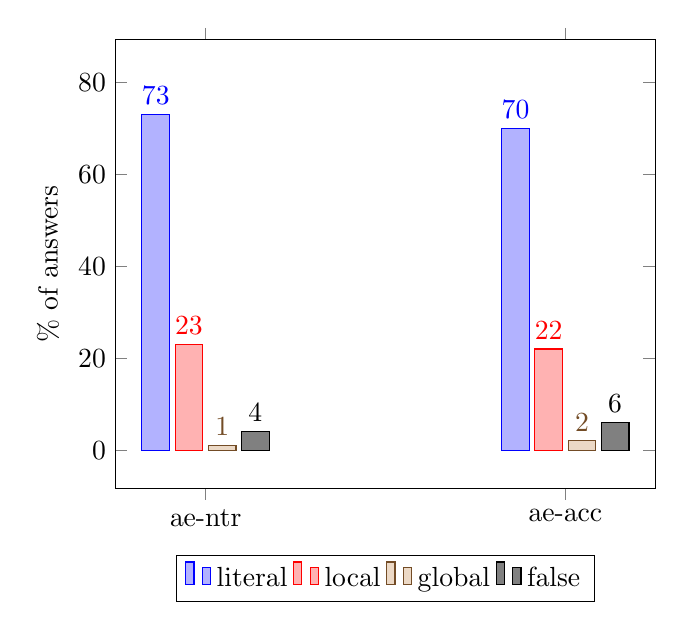
\begin{tikzpicture}

      \begin{axis}[ybar, enlargelimits=0.25, legend
        style={at={(0.5,-0.15)}, anchor=north, legend columns=-1},
        ylabel={\% of answers}, symbolic x
        coords={ae-ntr,dummy,ae-acc}, xtick=data, nodes
        near coords, nodes near coords align={vertical}, ymin = 8 ]

        \addplot coordinates {(ae-ntr,73) (ae-acc,70)};

        \addplot coordinates {(ae-ntr,23) (ae-acc,22)};

        \addplot coordinates {(ae-ntr,1) (ae-acc,2)};

        \addplot coordinates {(ae-ntr,4) (ae-acc,6)};

        % \addplot coordinates {(ae-ntr,83) (ae-acc,80) (ge-ntr,53)
        % (ge-acc,56)};

        % \addplot coordinates {(ae-ntr,26) (ae-acc,25) (ge-ntr,33)
        % (ge-acc,26)};

        % \addplot coordinates {(ae-ntr,1) (ae-acc,2) (ge-ntr,0)
        % (ge-acc,1)};

        % \addplot coordinates {(ae-ntr,4) (ae-acc,7) (ge-ntr,28)
        % (ge-acc,31)};

        \legend{literal, local, global, false}

      \end{axis}

    \end{tikzpicture}
  \end{center}
\end{frame}

\begin{frame}
  \frametitle{Results \GE-Condition \hfill (answer types)}
  \begin{center}
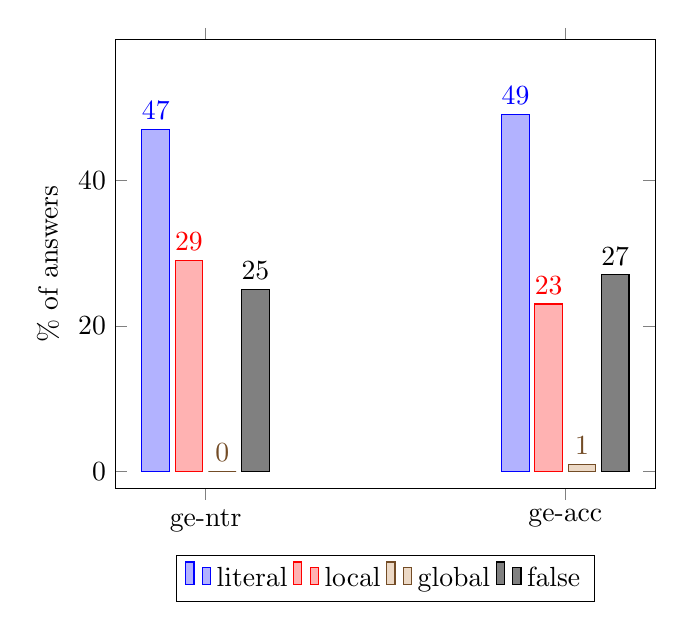
\begin{tikzpicture}

  \begin{axis}[ybar, 
               enlargelimits=0.25, 
               legend style={at={(0.5,-0.15)},
                 anchor=north,
                 legend columns=-1}, 
               ylabel={\% of answers}, 
               symbolic x coords={ge-ntr,dummy,ge-acc}, 
               xtick=data,
               nodes near coords,
               nodes near coords align={vertical},
               ymin = 8
               ]

    \addplot coordinates {(ge-ntr,47) (ge-acc,49)}; 

    \addplot coordinates {(ge-ntr,29) (ge-acc,23)}; 

    \addplot coordinates {(ge-ntr,0) (ge-acc,1)};

    \addplot coordinates {(ge-ntr,25) (ge-acc,27)};

    % \addplot coordinates {(ae-ntr,83) (ae-acc,80) (ge-ntr,53) (ge-acc,56)}; 

    % \addplot coordinates {(ae-ntr,26) (ae-acc,25) (ge-ntr,33) (ge-acc,26)}; 

    % \addplot coordinates {(ae-ntr,1) (ae-acc,2) (ge-ntr,0) (ge-acc,1)};

    % \addplot coordinates {(ae-ntr,4) (ae-acc,7) (ge-ntr,28) (ge-acc,31)};

    \legend{literal, local, global, false}

  \end{axis}

\end{tikzpicture}

  \end{center}
\end{frame}


\begin{frame}
  \frametitle{Results \AE-Condition \hfill (subject types)}
  \begin{center}
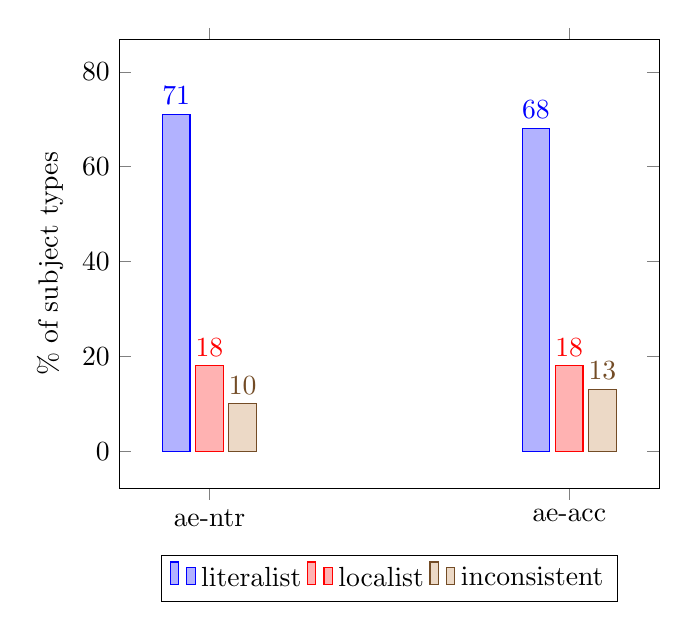
\begin{tikzpicture}

  \begin{axis}[ybar, 
               enlargelimits=0.25, 
               legend style={at={(0.5,-0.15)},
                 anchor=north,
                 legend columns=-1}, 
               ylabel={\% of subject types}, 
               symbolic x coords={ae-ntr,dummy,ae-acc}, 
               xtick=data,
               nodes near coords,
               nodes near coords align={vertical},
               ymin = 8
               ]

    \addplot coordinates {(ae-ntr,71) (ae-acc,68)}; 

    \addplot coordinates {(ae-ntr,18) (ae-acc,18)}; 

    \addplot coordinates {(ae-ntr,10) (ae-acc,13)};

    % \addplot coordinates {(ae-ntr,83) (ae-acc,80) (ge-ntr,53) (ge-acc,56)}; 

    % \addplot coordinates {(ae-ntr,26) (ae-acc,25) (ge-ntr,33) (ge-acc,26)}; 

    % \addplot coordinates {(ae-ntr,1) (ae-acc,2) (ge-ntr,0) (ge-acc,1)};

    % \addplot coordinates {(ae-ntr,4) (ae-acc,7) (ge-ntr,28) (ge-acc,31)};

    \legend{literalist, localist, inconsistent}

  \end{axis}

\end{tikzpicture}

  \end{center}
\end{frame}


\begin{frame}
  \frametitle{Results \GE-Condition \hfill (subject types)}
    \begin{center}
      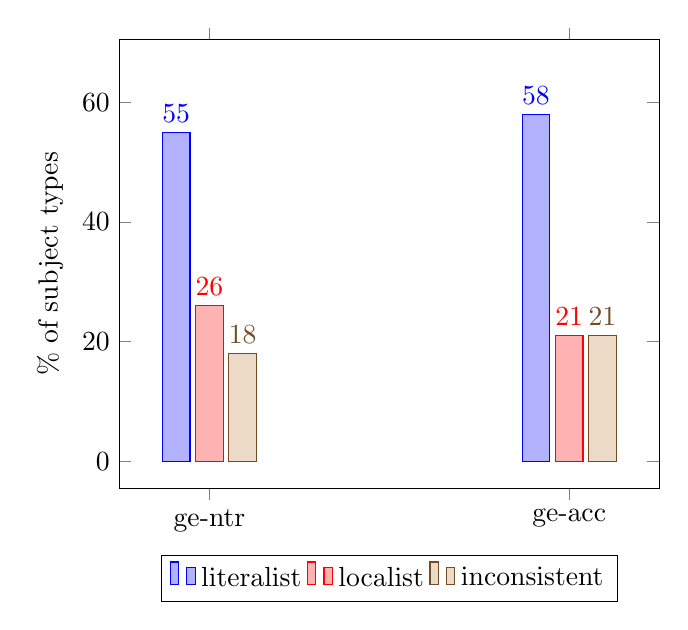
\begin{tikzpicture}

  \begin{axis}[ybar, 
               enlargelimits=0.25, 
               legend style={at={(0.5,-0.15)},
                 anchor=north,
                 legend columns=-1}, 
               ylabel={\% of subject types}, 
               symbolic x coords={ge-ntr,dummy,ge-acc}, 
               xtick=data,
               nodes near coords,
               nodes near coords align={vertical},
               ymin = 8
               ]

    \addplot coordinates {(ge-ntr,55) (ge-acc,58)}; 

    \addplot coordinates {(ge-ntr,26) (ge-acc,21)}; 

    \addplot coordinates {(ge-ntr,18) (ge-acc,21)};

    % \addplot coordinates {(ae-ntr,83) (ae-acc,80) (ge-ntr,53) (ge-acc,56)}; 

    % \addplot coordinates {(ae-ntr,26) (ae-acc,25) (ge-ntr,33) (ge-acc,26)}; 

    % \addplot coordinates {(ae-ntr,1) (ae-acc,2) (ge-ntr,0) (ge-acc,1)};

    % \addplot coordinates {(ae-ntr,4) (ae-acc,7) (ge-ntr,28) (ge-acc,31)};

    \legend{literalist, localist, inconsistent}

  \end{axis}

\end{tikzpicture}

    \end{center}
\end{frame}




\begin{frame}
  \frametitle{Comparing \AE\ and \GE\ Subject Types}

  \begin{center}
    \begin{tabular}{lccc}
      & \multicolumn{3}{c}{ge-ntr} \\ \cmidrule(r){2-4}
      ae-ntr & literalist & localist & inconsistent \\ \midrule
      literalist   & 19 & 2 & 6\\
      localist     &  0 & 7 & 0 \\
      inconsistent &  2 & 1 & 1\\
    \end{tabular}
  \end{center}

  \medskip

  \begin{center}
    \begin{tabular}{lccc}
      & \multicolumn{3}{c}{ge-acc} \\ \cmidrule(r){2-4}
      ae-acc & literalist & localist & inconsistent \\ \midrule
      literalist   & 19 & 2 & 5\\
      localist     &  0 & 5 & 2 \\
      inconsistent &  3 & 1 & 1\\
    \end{tabular}
  \end{center}

\end{frame}


\begin{frame}
  \frametitle{Tentative Naive Conclusions}
  
  \begin{block}{Availability of Readings}
    \begin{itemize}
    \item most subjects applied a literal reading (consistently)
    \item some subjects applied a local reading (consistently)
    \item few global answers, none applied consistently
    \end{itemize}
  \end{block}

  \begin{block}{Effect of Prosody}
    \begin{itemize}
    \item prosody does not seem to any effect
    \end{itemize}
  \end{block}

  \begin{block}{Open Issue}
    \begin{itemize}
    \item how to interpret data from visually-incremental
      \acro{tv}-task?
    \end{itemize}

  \end{block}
\end{frame}

\begin{frame}
  \frametitle{Target-Related Fillers}
  \begin{block}{Motivation}
    \begin{itemize}
    \item use ambiguous sentences with a clearly preferred reading
    \item investigate conditions where preferred reading can be judged
      true or false first or second
    \item[$\Rightarrow$] do we see both readings in the visually-incremental
      \acro{tv}-task?
    \item[$\Rightarrow$] do we see evidence of the preference?
    \end{itemize}
  \end{block}
\end{frame}

\begin{frame}
  \frametitle{Target-Related Fillers}
  \begin{block}{Sentence Material: Late-/Early-Closure Ambiguity}
    \begin{exe}
      \ex The letter is connected with circles and squares with
        suns.
        \begin{xlist}
          \ex The bell is connected with circles and squares; the latter
            but not the former contain suns. \hfill (\LC)
          \ex The bell is connected with circles and squares; both
            contain suns. \hfill (\EC)
        \end{xlist}
    \end{exe}
  \end{block}

  \begin{center}
    \includegraphics[width=0.35\textwidth]{../../pictures/LC-EC-Contrast.png}
  \end{center}

\end{frame}

\begin{frame}
  \frametitle{Target-Related Fillers}

  \begin{block}{Conditions}
    \begin{center}
      \begin{tabular}{lccc}
        & \multicolumn{3}{c}{prosodical cue} \\ \cmidrule(r){2-4}
        1$^{\mathrm{st}}$ in sequence & neutral & \LC & \EC \\ \midrule
        \LC & e-ntr & l-l & l-e \\
        \EC & e-ntr & e-l & e-e \\
      \end{tabular}
    \end{center}
  \end{block}

  \begin{block}{Prosodical Cues}
    \begin{itemize}
      \item[ntr:] The letter is connected with circles and squares with
        suns.
      \item[LC:] The letter is connected with circles \# and squares with
        suns.
      \item[EC:] The letter is connected with circles and squares \# with
        suns.
    \end{itemize}
  \end{block}

\end{frame}

\begin{frame}
  \frametitle{\LC-Sequence}
  \begin{center}
    ``Die Schere ist mit Kreisen und Vierecken mit Sonnen verbunden.''

    \vspace{0.1cm}

    \includegraphics[width=0.5 \textwidth]{../../pictures/lc_01_1.pdf}

    \vspace{0.1cm}

    \begin{multicols}{3}
      \begin{itemize} 
      \item[$\Box$] True\\
        \onslide<2>{$\leadsto$  \mymark{false}}
      \item[$\Box$] False\\
        \onslide<2>{$\leadsto$ \mymark{false}}
      \item[$\Box$] Need more info 
      \end{itemize}
    \end{multicols}

  \end{center}
\end{frame}


\begin{frame}
  \frametitle{\LC-Sequence}
  \begin{center}
    ``Die Schere ist mit Kreisen und Vierecken mit Sonnen verbunden.''

    \vspace{0.1cm}

    \includegraphics[width=0.5 \textwidth]{../../pictures/lc_01_2.pdf}

    \vspace{0.1cm}

    \begin{multicols}{3}
      \begin{itemize} 
      \item[$\Box$] True\\
        \onslide<2>{$\leadsto$  \mymark{false}}
      \item[$\Box$] False\\
        \onslide<2>{$\leadsto$ \mymark{false}}
      \item[$\Box$] Need more info 
      \end{itemize}
    \end{multicols}

  \end{center}
\end{frame}


\begin{frame}
  \frametitle{\LC-Sequence}
  \begin{center}
    ``Die Schere ist mit Kreisen und Vierecken mit Sonnen verbunden.''

    \vspace{0.1cm}

    \includegraphics[width=0.5 \textwidth]{../../pictures/lc_01_3.pdf}

    \vspace{0.1cm}

    \begin{multicols}{3}
      \begin{itemize} 
      \item[$\Box$] True\\
        \onslide<2>{$\leadsto$  \mymark{LC}}
      \item[$\Box$] False\\
        \onslide<2>{$\leadsto$ \mymark{false}}
      \item[$\Box$] Need more info 
      \end{itemize}
    \end{multicols}

  \end{center}
\end{frame}
\begin{frame}
  \frametitle{\LC-Sequence}
  \begin{center}
    ``Die Schere ist mit Kreisen und Vierecken mit Sonnen verbunden.''

    \vspace{0.1cm}

    \includegraphics[width=0.5 \textwidth]{../../pictures/lc_01_4.pdf}

    \vspace{0.1cm}

    \begin{multicols}{3}
      \begin{itemize} 
      \item[$\Box$] True\\
        \onslide<2>{$\leadsto$  \mymark{false}}
      \item[$\Box$] False\\
        \onslide<2>{$\leadsto$ \mymark{false}}
      \item[$\Box$] Need more info 
      \end{itemize}
    \end{multicols}

  \end{center}
\end{frame}

\begin{frame}
  \frametitle{\LC-Sequence}
  \begin{center}
    ``Die Schere ist mit Kreisen und Vierecken mit Sonnen verbunden.''

    \vspace{0.1cm}

    \includegraphics[width=0.5 \textwidth]{../../pictures/lc_01_5.pdf}

    \vspace{0.1cm}

    \begin{multicols}{3}
      \begin{itemize} 
      \item[$\Box$] True\\
        \onslide<2>{$\leadsto$  \mymark{false}}
      \item[$\Box$] False\\
        \onslide<2>{$\leadsto$ \mymark{false}}
      \item[$\Box$] Need more info 
      \end{itemize}
    \end{multicols}

  \end{center}
\end{frame}

\begin{frame}
  \frametitle{\LC-Sequence}
  \begin{center}
    ``Die Schere ist mit Kreisen und Vierecken mit Sonnen verbunden.''

    \vspace{0.1cm}

    \includegraphics[width=0.5 \textwidth]{../../pictures/lc_01_6.pdf}

    \vspace{0.1cm}

    \begin{multicols}{3}
      \begin{itemize} 
      \item[$\Box$] True\\
        \onslide<2>{$\leadsto$  \mymark{false}}
      \item[$\Box$] False\\
        \onslide<2>{$\leadsto$ \mymark{EC}}
      \item[$\Box$] Need more info 
      \end{itemize}
    \end{multicols}

  \end{center}
\end{frame}

\begin{frame}
  \frametitle{\LC-Sequence}
  \begin{center}
    ``Die Schere ist mit Kreisen und Vierecken mit Sonnen verbunden.''

    \vspace{0.1cm}

    \includegraphics[width=0.5 \textwidth]{../../pictures/lc_01_7.pdf}

    \vspace{0.1cm}

    \begin{multicols}{3}
      \begin{itemize} 
      \item[$\Box$] True\\
        \onslide<2>{$\leadsto$  \mymark{false}}
      \item[$\Box$] False\\
        \onslide<2>{$\leadsto$ \mymark{false}}
      \item[$\Box$] Need more info 
      \end{itemize}
    \end{multicols}

  \end{center}
\end{frame}

\begin{frame}
  \frametitle{\EC-Sequence}
  \begin{center}
    ``Die Schere ist mit Kreisen und Vierecken mit Sonnen verbunden.''

    \vspace{0.1cm}

    \includegraphics[width=0.5 \textwidth]{../../pictures/ec_01_1.pdf}

    \vspace{0.1cm}

    \begin{multicols}{3}
      \begin{itemize} 
      \item[$\Box$] True\\
        \onslide<2>{$\leadsto$  \mymark{false}}
      \item[$\Box$] False\\
        \onslide<2>{$\leadsto$ \mymark{false}}
      \item[$\Box$] Need more info 
      \end{itemize}
    \end{multicols}

  \end{center}
\end{frame}


\begin{frame}
  \frametitle{\EC-Sequence}
  \begin{center}
    ``Die Schere ist mit Kreisen und Vierecken mit Sonnen verbunden.''

    \vspace{0.1cm}

    \includegraphics[width=0.5 \textwidth]{../../pictures/ec_01_2.pdf}

    \vspace{0.1cm}

    \begin{multicols}{3}
      \begin{itemize} 
      \item[$\Box$] True\\
        \onslide<2>{$\leadsto$  \mymark{false}}
      \item[$\Box$] False\\
        \onslide<2>{$\leadsto$ \mymark{false}}
      \item[$\Box$] Need more info 
      \end{itemize}
    \end{multicols}

  \end{center}
\end{frame}


\begin{frame}
  \frametitle{\EC-Sequence}
  \begin{center}
    ``Die Schere ist mit Kreisen und Vierecken mit Sonnen verbunden.''

    \vspace{0.1cm}

    \includegraphics[width=0.5 \textwidth]{../../pictures/ec_01_3.pdf}

    \vspace{0.1cm}

    \begin{multicols}{3}
      \begin{itemize} 
      \item[$\Box$] True\\
        \onslide<2>{$\leadsto$  \mymark{false}}
      \item[$\Box$] False\\
        \onslide<2>{$\leadsto$ \mymark{EC}}
      \item[$\Box$] Need more info 
      \end{itemize}
    \end{multicols}

  \end{center}
\end{frame}


\begin{frame}
  \frametitle{\EC-Sequence}
  \begin{center}
    ``Die Schere ist mit Kreisen und Vierecken mit Sonnen verbunden.''

    \vspace{0.1cm}

    \includegraphics[width=0.5 \textwidth]{../../pictures/ec_01_4.pdf}

    \vspace{0.1cm}

    \begin{multicols}{3}
      \begin{itemize} 
      \item[$\Box$] True\\
        \onslide<2>{$\leadsto$  \mymark{false}}
      \item[$\Box$] False\\
        \onslide<2>{$\leadsto$ \mymark{false}}
      \item[$\Box$] Need more info 
      \end{itemize}
    \end{multicols}

  \end{center}
\end{frame}


\begin{frame}
  \frametitle{\EC-Sequence}
  \begin{center}
    ``Die Schere ist mit Kreisen und Vierecken mit Sonnen verbunden.''

    \vspace{0.1cm}

    \includegraphics[width=0.5 \textwidth]{../../pictures/ec_01_5.pdf}

    \vspace{0.1cm}

    \begin{multicols}{3}
      \begin{itemize} 
      \item[$\Box$] True\\
        \onslide<2>{$\leadsto$  \mymark{LC}}
      \item[$\Box$] False\\
        \onslide<2>{$\leadsto$ \mymark{false}}
      \item[$\Box$] Need more info 
      \end{itemize}
    \end{multicols}

  \end{center}
\end{frame}

\begin{frame}
  \frametitle{Results \LC-Condition \hfill (answer types)}

  \begin{center}

    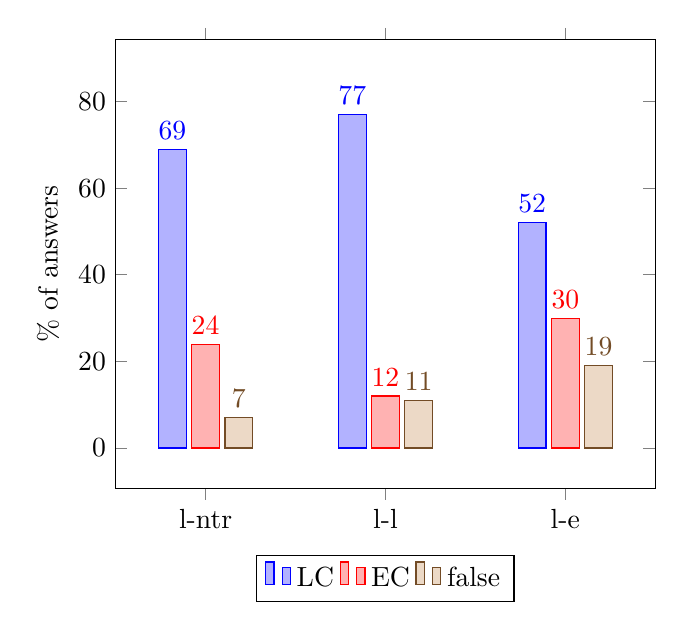
\begin{tikzpicture}

  \begin{axis}[ybar, 
               enlargelimits=0.25, 
               legend style={at={(0.5,-0.15)},
                 anchor=north,
                 legend columns=-1}, 
               ylabel={\% of answers}, 
               symbolic x coords={l-ntr,l-l,l-e}, 
               xtick=data,
               nodes near coords,
               nodes near coords align={vertical},
               ymin = 8
               ]

    \addplot coordinates {(l-ntr, 69) (l-l, 77) (l-e, 52)}; 

    \addplot coordinates {(l-ntr, 24) (l-l, 12) (l-e, 30)}; 

    \addplot coordinates {(l-ntr, 7) (l-l, 11) (l-e, 19)}; 

    % \addplot coordinates {(l-ntr, 93) (l-l, 101) (l-e, 70) (e-ntr, 85)
    %   (e-l, 100) (e-e, 75)}; 

    % \addplot coordinates {(l-ntr, 33) (l-l, 16) (l-e, 40) (e-ntr, 34)
    %   (e-l, 16) (e-e, 43)}; 

    % \addplot coordinates {(l-ntr, 9) (l-l, 14) (l-e, 25) (e-ntr, 16)
    %   (e-l, 15) (e-e, 17)}; 

    \legend{LC, EC, false}

  \end{axis}

\end{tikzpicture}

    
  \end{center}
\end{frame}



\begin{frame}
  \frametitle{Results \EC-Condition \hfill (answer types)}

  \begin{center}

    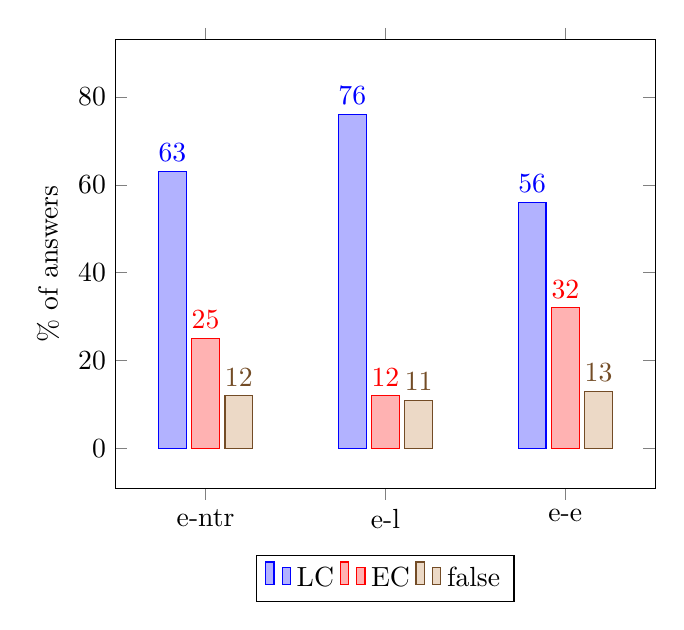
\begin{tikzpicture}

  \begin{axis}[ybar, 
               enlargelimits=0.25, 
               legend style={at={(0.5,-0.15)},
                 anchor=north,
                 legend columns=-1}, 
               ylabel={\% of answers}, 
               symbolic x coords={e-ntr,e-l,e-e,}, 
               xtick=data,
               nodes near coords,
               nodes near coords align={vertical},
               ymin = 8
               ]

    \addplot coordinates {(e-ntr, 63)
      (e-l, 76) (e-e, 56)}; 

    \addplot coordinates {(e-ntr, 25)
      (e-l, 12) (e-e, 32)}; 

    \addplot coordinates {(e-ntr, 12)
      (e-l, 11) (e-e, 13)}; 

    % \addplot coordinates {(l-ntr, 93) (l-l, 101) (l-e, 70) (e-ntr, 85)
    %   (e-l, 100) (e-e, 75)}; 

    % \addplot coordinates {(l-ntr, 33) (l-l, 16) (l-e, 40) (e-ntr, 34)
    %   (e-l, 16) (e-e, 43)}; 

    % \addplot coordinates {(l-ntr, 9) (l-l, 14) (l-e, 25) (e-ntr, 16)
    %   (e-l, 15) (e-e, 17)}; 

    \legend{LC, EC, false}

  \end{axis}

\end{tikzpicture}

    
  \end{center}
\end{frame}

\begin{frame}
  \frametitle{Results \LC-Condition \hfill (subject types)}

  \begin{center}

    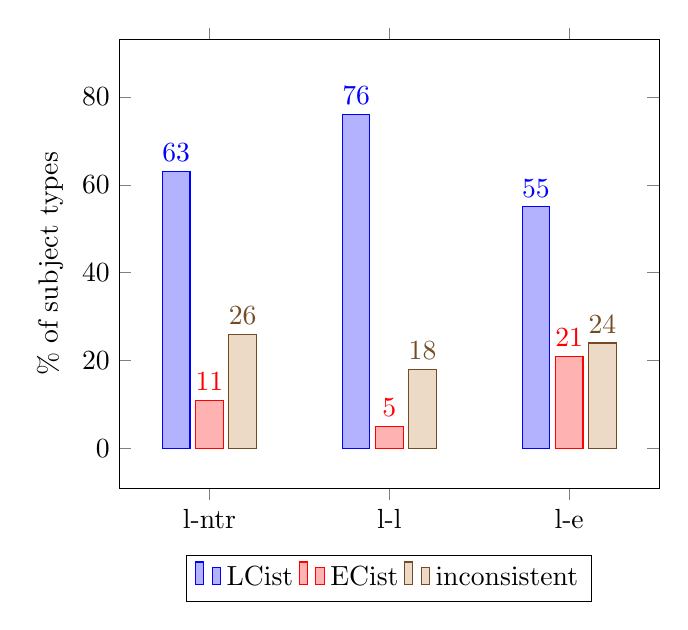
\begin{tikzpicture}

  \begin{axis}[ybar, 
               enlargelimits=0.25, 
               legend style={at={(0.5,-0.15)},
                 anchor=north,
                 legend columns=-1}, 
               ylabel={\% of subject types}, 
               symbolic x coords={l-ntr,l-l,l-e}, 
               xtick=data,
               nodes near coords,
               nodes near coords align={vertical},
               ymin = 8
               ]

    \addplot coordinates {(l-ntr, 63) (l-l, 76) (l-e, 55)}; 

    \addplot coordinates {(l-ntr, 11) (l-l, 5) (l-e, 21)}; 

    \addplot coordinates {(l-ntr, 26) (l-l, 18) (l-e, 24)}; 

    % \addplot coordinates {(l-ntr, 93) (l-l, 101) (l-e, 70) (e-ntr, 85)
    %   (e-l, 100) (e-e, 75)}; 

    % \addplot coordinates {(l-ntr, 33) (l-l, 16) (l-e, 40) (e-ntr, 34)
    %   (e-l, 16) (e-e, 43)}; 

    % \addplot coordinates {(l-ntr, 9) (l-l, 14) (l-e, 25) (e-ntr, 16)
    %   (e-l, 15) (e-e, 17)}; 

    \legend{LCist, ECist, inconsistent}

  \end{axis}

\end{tikzpicture}

    
  \end{center}
\end{frame}

\begin{frame}
  \frametitle{Results \EC-Condition \hfill (subject types)}

  \begin{center}

    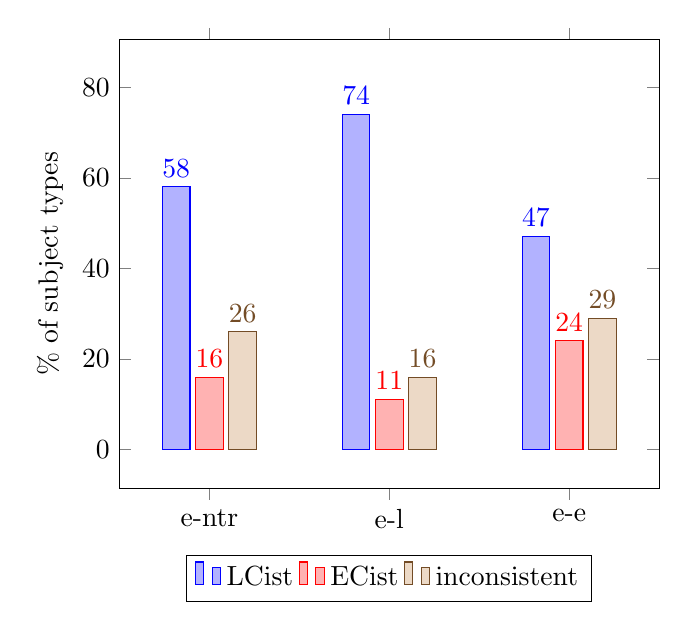
\begin{tikzpicture}

  \begin{axis}[ybar, 
               enlargelimits=0.25, 
               legend style={at={(0.5,-0.15)},
                 anchor=north,
                 legend columns=-1}, 
               ylabel={\% of subject types}, 
               symbolic x coords={e-ntr,e-l,e-e,}, 
               xtick=data,
               nodes near coords,
               nodes near coords align={vertical},
               ymin = 8
               ]

    \addplot coordinates {(e-ntr, 58)
      (e-l, 74) (e-e, 47)}; 

    \addplot coordinates {(e-ntr, 16)
      (e-l, 11) (e-e, 24)}; 

    \addplot coordinates {(e-ntr, 26)
      (e-l, 16) (e-e, 29)}; 

    % \addplot coordinates {(l-ntr, 93) (l-l, 101) (l-e, 70) (e-ntr, 85)
    %   (e-l, 100) (e-e, 75)}; 

    % \addplot coordinates {(l-ntr, 33) (l-l, 16) (l-e, 40) (e-ntr, 34)
    %   (e-l, 16) (e-e, 43)}; 

    % \addplot coordinates {(l-ntr, 9) (l-l, 14) (l-e, 25) (e-ntr, 16)
    %   (e-l, 15) (e-e, 17)}; 

    \legend{LCist, ECist, inconsistent}

  \end{axis}

\end{tikzpicture}
    
  \end{center}
\end{frame}


\begin{frame}
  \frametitle{Tentative Naive Conclusions}
  \begin{block}{Lessons from the \LC-\EC-Conditions}
    \begin{itemize}
    \item both \LC- and \EC-readings show up 
    \item the preference for \LC-readings shows in more \LC-answers
    \item all of this is irrespective of position
    \item prosody does seem to have the expected effect
    \end{itemize}
  \end{block}

  \begin{block}{Embedded Implicatures?!?}
    \begin{itemize}
    \item proper statistical analysis is pending, but \dots
    \item \dots it appears that local readings exist but are dispreferred
    \end{itemize}
  \end{block}
\end{frame}



\begin{frame}[plain,allowframebreaks]
  \begin{block}{References}
    \printbibliography[heading=subbibliography]
  \end{block}
\end{frame}
\end{document}


\appendix

\begin{frame}
  \frametitle{Results \AE-Condition}
  \begin{center}
    \includegraphics[width=0.7\textwidth]{../../pictures/ae-ntr.png}

    \vspace{0.2cm}
    \# of true/false judgements on positions in ae-ntr
  \end{center}
\end{frame}

\begin{frame}
  \frametitle{Results \AE-Condition}
  \begin{center}
    \includegraphics[width=0.7\textwidth]{../../pictures/ae-acc.png}

    \vspace{0.2cm}
    \# of true/false judgements on positions in ae-acc
  \end{center}
\end{frame}

\begin{frame}
  \frametitle{Results \GE-Condition}
  \begin{center}
    \includegraphics[width=0.7\textwidth]{../../pictures/ge-ntr.png}

    \vspace{0.2cm}
    \# of true/false judgements on positions in ge-ntr
  \end{center}
\end{frame}

\begin{frame}
  \frametitle{Results \GE-Condition}
  \begin{center}
    \includegraphics[width=0.7\textwidth]{../../pictures/ge-acc.png}

    \vspace{0.2cm}
    \# of true/false judgements on positions in ge-acc
  \end{center}
\end{frame}

